\documentclass[UTF8]{article}
\usepackage{amsmath,amssymb,amsthm}
\usepackage{ctex}
\usepackage{graphicx}
\usepackage{float}


\newcommand{\D}{\mathrm{d}}
\newcommand{\E}{\mathrm{e}}
\newcommand{\im}{\mathrm{i}}


\begin{document}
	
\section*{0 小振动}

在这一章里如果没有求和号就是使用爱因斯坦求和约定.

\subsection*{0 多自由度力学体系的谐振}

	考虑一个有$n$个自由度的保守力学系统,其拉格朗日量为$L(q_i,\dot{q}_i)=T-V$,势能$V(q_i)$.其中$q_i,\dot{q_i}$是广义坐标和广义速度.
	
	这里我们感兴趣的是在稳定的平衡位置附近的运动.设系统的一个平衡位置为$q_{i0}$,则必有
	
	\[\left.\frac{\partial V}{\partial q_i}\right|_{q_i=q_{i0}}=0\]
	
	不妨把广义坐标齐次化,令$x_i:=q_i-q_{i0}$,则:
	
	\[\left.\frac{\partial V}{\partial x_i}\right|_{x_i=0}=0\]
	
	那么在平衡位置附近可以将势能进行Taylor展开
	
	\[V(x)=V_0+\frac{1}{2}k_{ij}x_ix_j+o(|x|^2)\]
	
	设$x=x_ie_i$,那么也可以写成矩阵的形式
	
	\[V(x)=V_0+\frac12x^Tkx\]
	
	而动能$T$本身就是$\dot{x}$的二次型$T=\frac12\dot{x}^Tm\dot{x}$,我们关心的运动的性质也足够良好以至于$\dot{x}$也是小量,故可取$m$为平衡位置的取值.
	
	那么系统的拉格朗日函数即
	
	\[L=\frac12(\dot{x}^Tm\dot{x}-x^Tkx)\]
	
	对应的动力学方程
	
	\[m_{ij}\ddot{x_i}+k_{ij}x_i=0\]
	
	现在我们来讨论谐振动解的存在性与完备性.直接假设这个系统具有简谐振动形式的解$x=c\E^{\im \omega t}$.那么$\ddot{x}=-\omega^2 x$,动力学方程化为
	
	\[(k_{ij}-\omega^2m_{ij})c_i=0\]
	
	也即
	
	\[(k-\omega^2m)c=0\]
	
	这样我们将微分方程的求解转化为代数方程的求解,即上述$n$元方程组的求解.
	
	方程组有非零解要求系数行列式为0,即
	
	\[\det(k-\omega^2m)=0\]
	
	二次型的对称性要求$m,k$都是实对称矩阵,故一定存在正交矩阵$P$,使得
	
	\[P^TmP=\mathrm{diag}\{m_1,m_2,\cdots,m_n\}=M\quad\Leftrightarrow\quad m=PMP^T\]
	
	再记$D=\mathrm{diag}\{\sqrt{m_1},\sqrt{m_2},\cdots,\sqrt{m_n}\}$(假设$m_i\ne0$,$D$可逆,这要求动能在平衡点非退化).那么系数矩阵满足关系
	
	\[k-\omega^2m=PD(D^{-1T}P^TkPD^{-1}-\omega^2I)D^TP^T\]
	
	故必有
	
	\[\det(k-\omega^2m)=m_1m_2\cdots m_n\det(D^{-1T}P^TkPD^{-1}-\omega^2I)\]

	注意到$D^{-1T}P^TkPD^{-1}$也是实对称矩阵,故其可以正交对角化(其实到这一步已经结束了),即存在正交矩阵$Q$,使得
	
	\[Q^T(D^{-1T}P^TkPD^{-1})Q=\mathrm{diag}\{\omega_1^2,\omega_2^2,\cdots\omega_n^2\}=\Omega\]
	
	平衡位置稳定要求$k$为正定矩阵,而合同变换不改变矩阵的正定性,所以$\omega_i^2$的记法是合理的.
	
	故
	
	\[k-\omega^2m=PDQ(\Omega-\omega^2I)Q^TD^TP^T\]
	
	\[\det(k-\omega^2m)=m_1m_2\cdots m_n\det(\Omega-\omega^2I)\]
	
	(说实话写到这里我突然意识到这不就是线代上的正定矩阵与实对称矩阵的同时对角化问题吗......失败大学生石锤了orz)
	
	上述推导表明$(k-\omega^2m)c=0$等价于$(\Omega-\omega^2I)Q^TD^TP^Tc=0$.再进行非退化代换$C=Q^TD^TP^Tc$,则等价于$(\Omega-\omega^2I)C=0$.
	
	而每一个特征向量对应$\cos\omega t$和$\sin \omega t$二线性无关解.记这些特征向量为系统的简正坐标$Q_i=C_{ij}x_j$.
	
	可见,在非退化的情况下,系统的确存在$2n$个线性无关的振动解,并且具有不超过$n$个共振频率.考虑到该线性常微分方程组解空间的维数只有$2n$,我们这里找到了系统的通解.
	
	至于具体的振动模式/特征向量(\textbf{简正模})的求解,从上面的推导可以看出直接按照线性代数中求解矩阵特征值与特征向量的解法即可.顺便提一下,由于奇奇怪怪的历史原因,刚刚出现的特征方程$|\omega^2m-k|=0$和物理上出现的其他类似的特征方程都叫\textbf{久期方程},至于为什么,向最近的记录神甫提问吧(逃)
	
	\newpage
	
	
	
	
	
	
	
	\subsection*{1 摄动法求解非谐振子}
	
	虽然上面得到了很优美的结论,但是我们不应忘记这是在Taylor展开取一阶项的条件下得到的.从一般的振动的意义下,这可以说是trivial而不符合万机之神精妙的创造(雾)的.对于振幅较大而非线性效应不可忽略的情况,我们也应予讨论.
	
	但在这之前,我们先来点数学(并不)上的铺垫:微扰法.
	
	举一个简单的例子(这是归纳法!科学方法!):考虑如下方程的求根
	
	\[x-1-\varepsilon x^3,\quad\varepsilon\ll1\]
	
	我们考虑求其在$x=1$附近的根,显然这是$\varepsilon$的函数.根据机械教圣典物理篇万物皆可Taylor的教义,我们将其展开为Taylor级数
	
	\[x=x^{(0)}+x^{(1)}\varepsilon+x^{(2)}\varepsilon^2+\cdots\]

	然后我们把这个级数代回到原方程,根据Taylor展开的唯一性比较$\varepsilon$对应项的系数,我们就可以得到一系列的方程,进而以任意高的精度解出$x^{(n)}$.
	
	具体操作上,显然零阶下有$x^{(0)}=1$.那么接下来我们保留到一阶项,代入得
	
	\[x^{(1)}\varepsilon-\varepsilon=0 \Rightarrow x^{(1)}=1\]
	
	计算出一阶项后,再保留到二阶项,得
	
	\[x^{(2)}\varepsilon^2-3\varepsilon^2=0\Rightarrow x^{(2)}=3\]
	
	以此类推,我们可以得出

	\begin{figure}[H]
		\centering
		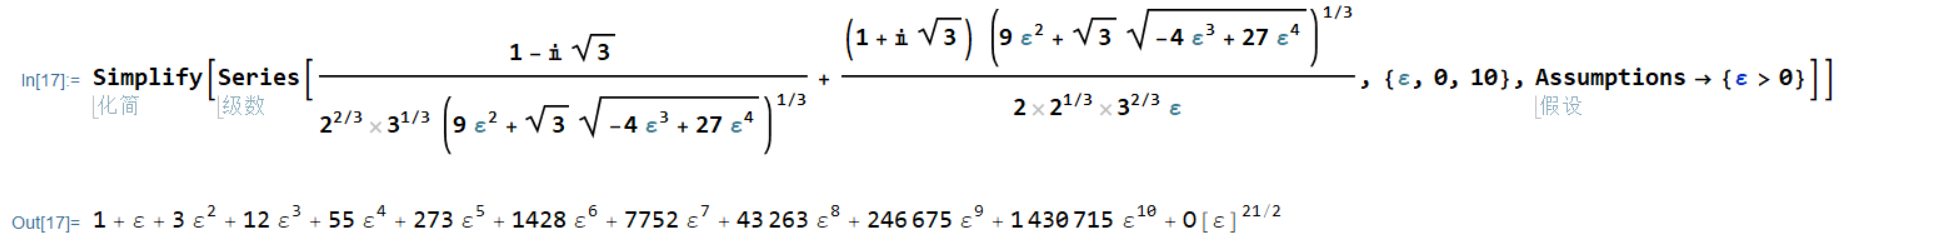
\includegraphics[width=1.25\linewidth]{pics/QQ截图20210720221755}
		\label{fig:qq20210720221755}
	\end{figure}
	
	(x)
	
	方程的另外两个跟当$\varepsilon\to 0$时趋于无穷,因而正则摄动(就是刚刚的操作)不适用,我们可以使用奇异摄动法来进行求解.具体来说,就是进行变量替换$x=\frac{\xi}{\varepsilon^\mu}$,代入方程可得
	
	\[\xi\varepsilon^{2\mu-1}-\varepsilon^{3\mu-1}-\xi^3=0\]
	
	考虑到$\varepsilon^{3\mu-1}$必然比其他两项小到不知哪里去了,舍去得
	
	\[\xi\varepsilon^{2\mu-1}-\xi^3=0\]
	
	回想起来我们进行这个变量代换的目的就是消掉$x$的发散,那么对机神的信仰告诉我们(?)$\xi(\varepsilon)$的零阶项必不为0.从而系数可能相等要求有$2\mu-1=0$,即$\mu=\frac{1}{2}$
	
	现在回到代换后的原始方程
	
	\[\xi-\varepsilon^{1/2}-\xi^3=0\]
	
	这个方程我们可以按照正则摄动进行展开求解(注意要按$\varepsilon^{1/2}$的幂次).一通操作后我们得到$x$的展开式(之一)
	
	\begin{figure}[H]
		\centering
		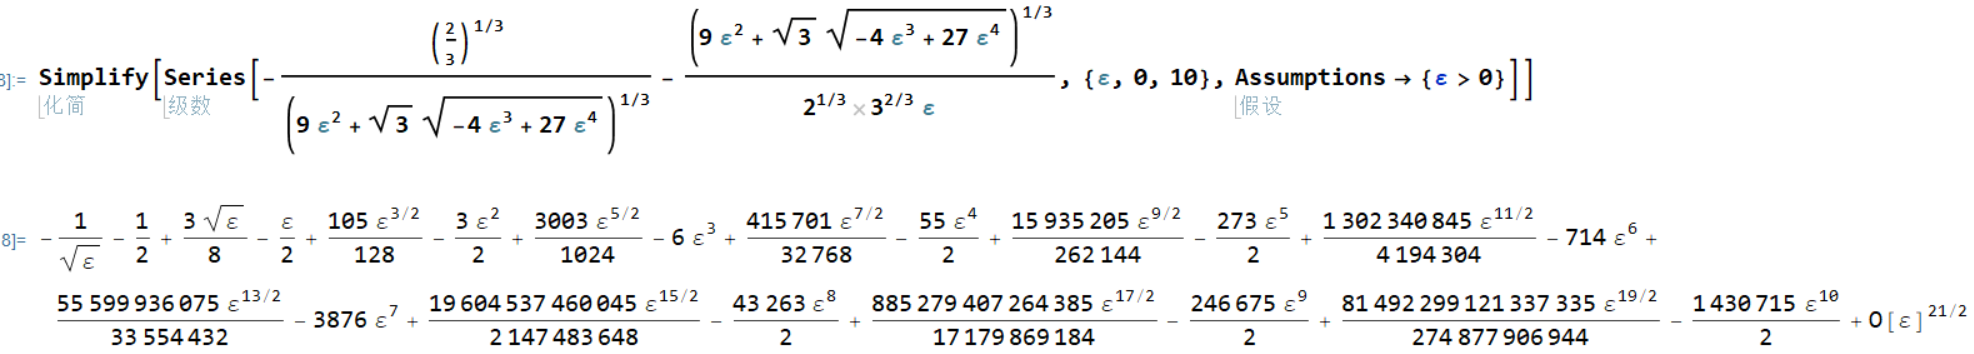
\includegraphics[width=1\linewidth]{pics/QQ截图20210720223418}
		\label{fig:qq20210720223418}
	\end{figure}
	
	至于什么收敛不收敛合法不合法的,那肯定是受了混沌的蛊惑对机神信仰不足才会发生的事,高阶的物理神甫甚至会使用渐近级数这种收敛到数学地狱里面的阴间操作,那么只好额叶切除了,请(悲)
	
	需要指出的是fx老师强调现代的计算机数值方法非常发达,而摄动法的收敛性与收敛速度也是有限的,如果你发现微扰摄动要算到几十几百项才能得到一个比较好的解........那你还是赶紧安抚一下计算机的机魂让他赶紧帮你算点数值解或者什么格点方法吧(悲)
	
	现在我们来考虑具体的动力学系统.不妨先考虑把一般情况下的拉格朗日函数展开到第一阶非线性项,也即三阶项.选取之前得到的简正坐标为广义坐标,那么拉格朗日函数具有如下形式:
	
	\[L=\frac12 (\dot{Q_i}^2-\omega_i^2Q_i^2)+\frac12 \lambda_{ijk}Q_i\dot{Q_j}\dot{Q_k}+\frac12 \mu_{ijk}Q_iQ_jQ_k\]
	
	并且对应的动力学方程满足如下形式
	
	\[\ddot{Q_i}+\omega_i^2Q_i=f(Q,\dot{Q},\ddot{Q})\]
	
	其中$f$为二次齐次函数.
	
	既然我们只将拉格朗日函数进行了额外的一次展开,我们就来求一阶修正:
	
	\[Q_i=Q_i^{(0)}+Q_i^{(1)}\]
	
	对这个神圣定义的解读是其中第一项为将$f$视为0的解,第二项为非线性因素引起的修正,且$Q_i^{(1)}\ll Q_i^{(0)}$.
	
	那么我们发现一阶项满足的方程
	
	\begin{align*}
		\ddot{Q_i}^{(1)}+\omega_i^2Q_i^{(1)}&=a_ia_j\cos(\omega_i t+\phi_i)\cos(\omega_j t+\phi)\\
		&=\frac12a_ia_j\{\cos[(\omega_i+\omega_j)t+(\phi_i+\phi_j)]+\cos[(\omega_i-\omega_j)t+(\phi_i-\phi_j)]\}
	\end{align*}
	
	可以看出非齐次项含有$\omega_i\pm\omega_j$项,也即一阶修正项中产生了系统固有频率和差的次级频率.这些频率称为\textbf{组合频率}.
	
	进一步我们可以考虑更高阶的修正.但是如果我们照搬上面的方法,不难发现二阶近似解中就会出现$\omega_i+\omega_j-\omega_i=\omega_i$项,解的振幅随时间增长,显然是不物理的.
	
	发生这种亵渎知识的事情,是因为刚刚的做法对欧姆尼赛亚的信仰不足(划掉)没有考虑高阶非线性项对本征频率的修正.
	
	这可以在一维系统的情况下考虑,力学中可以证明此时有界运动必然是周期性的,从而可以展开成基频对应的Fourier级数.然而如果忽略本征频率的改变,那么Fourier展开的条件被破坏,无法保证级数收敛到真实运动(事实上应该是一定不收敛?).所以在考虑高阶修正时必须从一开始就考虑本征频率的改变.
	
	不妨以一个一维的非谐振子为例.一般地,我们考虑一个光滑的势函数,将其在平衡位置对$x$展开成Taylor级数,则拉格朗日函数
	
	\[L=\frac{1}{2}m\dot{x}^2-\frac{1}{2}m\omega_0^2x^2-\sum_{n=3}^{\infty}\frac{1}{n+1}f_nx^{n+1}\]
	
	对应的动力学方程
	
	\[\ddot{x}+\omega_0^2x=-\sum_{n=2}^{\infty}f_nx^n\]
	
	(不会吧不会吧不会有人在这个跟field theory没有半毛钱关系的地方还要用Einstein求和吧)
	
	为了使用摄动法,我们考虑要以之进行展开的量.既然势能是对位移$x$进行展开的,我们应选取$x$的一个特征尺度为小量,如某种意义下的振幅.这样,用无量纲的$\varepsilon$标示小量的阶数,我们可以设初始条件
	
	\[x|_{t=0}=\varepsilon A,\quad\dot{x}|_{t=0}=0\]
	
	将$x$有展开成类似幂级数形式的解:
	
	\[x=\varepsilon x^{(1)}+\varepsilon^2 x^{(2)}+\varepsilon^3 x^{(3)}+\cdots\]
	
	显然$x^{(0)}=0,x^{(1)}=A\cos \omega t$.
	
	现在再将$\omega$展开:
	
	\[\omega=\omega^{(0)}+\varepsilon\omega^{(1)}+\varepsilon^2\omega^{(2)}+\cdots\]
	
	显然$\omega^{(0)}=\omega_0$.
	
	这时我们也将初始条件展开,可以得到
	
	\[x^{(1)}|_{t=0}=A,x^{(k)}|_{t=0}=0(k>1);\quad \dot{x}^{(k)}|_{t=0}=0(k>0)\]
	
	先保留到二阶小量(即$\varepsilon$的二次项),代入动力学方程,化简得:
	
	\[
		\begin{aligned}
			\ddot{x}^{(1)}+\omega_0^2 x^{(1)}
			&=-f_2A^2\cos^2\omega t+2\omega_0\omega^{(1)}A\cos\omega t\\
			&=-\frac{1}{2}f_2A^2-\frac{1}{2}f_2A^2\cos2\omega t+2\omega_0\omega^{(1)}A\cos\omega t
		\end{aligned}
	\]
	
	等式中不出现共振项(好像也叫久期项?不管了翻译出来挨打)要求$\omega^{(1)}=0$,与之前的讨论相符.于是现在二阶方程变为	
	
	\[\ddot{x}^{(2)}+\omega_0^2 x^{(2)}=-\frac{1}{2}f_2A^2-\frac{1}{2}f_2A^2\cos2\omega t\]
	
	相信不是物理学院的同学肯定都会解这个非齐次线性微分方程(物理学院的同学还没学orz!),随便用点Laplace变换或者什么方法很容易解出
	
	\[x^{(2)}=(-\frac{1}{2}+\frac{1}{3}\cos\omega+\frac{1}{6}\cos2\omega t)\frac{f_2A^2}{\omega_0^2}\]
	
	(这里Landau直接忽略了初始条件orz但是如果不忽视初始条件好像严格说要跑出个$\omega_0$?我也不清楚orz不过偷偷换成$\omega$了,至少在三阶近似下没影响到频移)
	
	接下来保留到三阶小量,注意到$x^{(1)}$的频移对三阶项无贡献,化简得
	
	\[
	\begin{aligned}
		\ddot{x}^{(3)}+\omega_0^2x^{(3)}=&-\frac{f_2^2A^3}{6\omega_0^2}(2-5\cos\omega t+2\cos2\omega t+\cos3\omega t)\\
		&-\frac{f_3A^3}{4}(3\cos\omega t+\cos3\omega t)+2A\omega_0\omega^{(2)}\cos\omega t
	\end{aligned}	
	\]
	
	令共振项系数为0,得
	
	\[\omega^{(2)}=\frac{5f_2^2A^2}{12\omega_0^3}-\frac{3f_3A^2}{8\omega_0}\]
	
	可见,高阶非线性效应使得系统的频率发生改变.并且频率与振幅有关,这是与线性谐振子非常不同的.
	
	这个计算我们还可以继续到任意阶的精度,考虑到继续计算意义不大,我们在此打住.
	
	由微扰摄动的计算过程可以看出,非线性效应对小振动的力学系统能够带来的一般影响有:
	
	\begin{enumerate}
		\item 系统固有频率改变,并且随振幅变化
		\item 系统的运动偏离简单的正弦函数,倍频的傅里叶系数不为0
	\end{enumerate}
	
	另外一个很好玩的现象是非线性谐振子的受迫振动,正好是cupt2021的一道题,具体而言就是一定驱动力大小时特定的驱动力频率下系统可能的受迫振动解的振幅不唯一,而分裂为3个分立的解,体现了欧姆尼赛亚创造的精妙,可以说是十分神奇的非线性现象了.具体可以参阅参考书\cite{Landau}29节.
	
	最后,我知道lc教授是一个非常敬业且水平极高的好老师,希望他能原谅我在这里yygq他的书(逃).
	
	\newpage





	
	
	\subsection*{10 参数共振}
	
	如果你对上面这个标题编号感觉奇怪,说明你还没有掌握神圣的二进制语,自裁,请(x)
	
	现在我们考虑另一种奇怪的谐振子,它的动力学方程可以写成如下形式:
	
	\[\ddot{x}+\omega^2(t)x=0)\]
	
	(不会吧不会吧不会有人在classical mechanics的范围还真的想Lagrangian从头做到尾吧?)
	
	如果$\omega(t)$是周期函数,那么这样的振子被称为参数振子(paramatric oscillator).设周期为$T$.
	
	注意到这是一个二阶常微分方程,那么它解空间的维数为2,也即存在两个线性无关的基本解$x_1,x_2$,并且二者的线性组合生成了方程的全部解.
	
	又由方程的平移对称性,$x_1(t+T),x_2(t+T)$也是方程的解,所以二者都可以由基本解线性表出.具体的表出系数取决于基的选取.通常的选取方法是所谓的标准基(standard basis):
	
	\[
	\begin{matrix}
		x_1(0)=1,&\dot{x_1}(0)=0\\
		x_2(0)=0,&\dot{x_1}(0)=1
	\end{matrix}
	\]
		
	在这种情况下,不难验证$(x_1(t+T),x_2(t+T))^T$由$(x_1(t),x_2(t))^T$表出的矩阵$R$(这称为Floquet矩阵/算符)具有简单的形式:
	
	\[
		\begin{pmatrix}
			x_1(t+T)
			\\x_2(t+T)
		\end{pmatrix}
		=
		\begin{pmatrix}
			x_1(T)&\dot{x_1}(T)\\
			x_2(T)&\dot{x_2}(T)
		\end{pmatrix}
		\cdot
		\begin{pmatrix}
			x_1(t)
			\\x_2(t)
		\end{pmatrix}
	\]
	
	即
	
	\[
		R=
		\begin{pmatrix}
			x_1(T)&\dot{x_1}(T)\\
			x_2(T)&\dot{x_2}(T)
		\end{pmatrix}
	\]
	
	这样,我们只要解出微分方程在$[0,t]$的解,就可以通过Floquet算符的重复作用以得到任意时间的$x$.
	
	为了研究Floquet算符幂次的性质,我们应求出其特征值.我们有本征方程
	
	\[\lambda^2-(x_1(T)+\dot{x}_2(T))\lambda+\det(R)=0\]
	
	注意到$\det(R)$就是解的Wronski行列式.根据常微分方程的Liouville定理,$W(T)=W(0)\exp(-\int_{0}^{T}p(x)\D x)=W(0)=1$,故本征方程

	\[\lambda^2-(x_1(T)+\dot{x}_2(T))\lambda+1=0\]
	
	这意味着二本征值的乘积为1.而$x_1(T)+\dot{x}_2(T)$则取决于$\omega(t)$的具体表现.从而我们可以讨论特征值的性质,进而讨论长时间下解的行为.至于怎么从$\omega(t)$确定$x_1(T)+\dot{x}_2(T)$,日后再说,问就是信仰不足(x)
	
	情况1:二本征值为共轭的单位圆上的复数.
	
	这对应着判别式小于0的情况,即$|x_1(T)+\dot{x}_2(T)|<2$.
	
	动动脑子(或者伺服颅骨)就知道这个时候两个解在$(-\infty,\infty)$上都是有界的,并且搞不好本征值对应的旋转的频率与$\omega$的频率满足一定比例那还可以直接出现周期解,trivial,trivial
	
	情况2:二本征值是不等的实数.
	
	这对应判别式大于0的情况.
	
	此时解空间中存在两个基函数,其中一个振幅按周期$T$指数增长,另一个指数衰减.
	
	情况3:二本征值简并,对应$x_1(T)+\dot{x}_2(T)=\pm2$.此时本征值必然为$\pm 1$.
	
	这种情况下$R$又分为可对角化与不可对角化两种情况.可对角化的作为第一种情况的退化,显然是trivial又trivial的,我们主要考虑不可对角化的情况.
	
	这时候Floquet算符在某组基下的矩阵为其Jordan标准型
	
	\[R=\begin{pmatrix}1&1\\0&1\end{pmatrix}\]

	作用n次后,有
	
	\[R^n=\begin{pmatrix}1&n\\0&1\end{pmatrix}\]

	也出现了无界的情况.也即解的振幅随时间线性发散,是第二种情况的退化.
	
	利用以上的讨论可以指导我们荡秋千,详见参考书\cite{LiuChuan}相应节的讨论.
	
	\newpage
	
	
	
	
	
	
	
\section*{1 刚体运动}
	
	这一节的讨论是经典到不能再经典的.具体的原因可以参见\cite{LiuChuan}P112的脚注.
	
\subsection*{0 转动的数学表述}
	
	刚体嘛,就是无穷多个满足$|x_i-x_j|=const,\forall i,j$的质点组.当然这不是很严谨的定义,但是大家都能理解,就意思一下,意会即可.
	
	绝大多数刚体有6个自由度.当然,也不是没有自由度少的,比如一维刚性杆的自由度就只有5,绕长轴旋转的自由度没了(当然你也可以说它还在,但是它也不参与任何相互作用,所以不如说它不存在)
	
	描述刚体运动时,我们常常会选择原点位于质心,一个与刚体一起运动,固连在刚体上的坐标架.这称为刚体的\textbf{体坐标架}(body axis).然而这并没什么卵用,加速度惯性力什么的麻烦的要死,所以我们一般只是意思意思,把一般参考系中的矢量投影到刚体坐标系的基上来方便表述而已.
	
	讨论转动时,可以采用两种等价的描述:一种视为矢量本身不变,而转动空间的基矢,相当于在空间中进行基变换(所谓的旋转矩阵就是过渡矩阵的转置),这称为被动观点;另一种是直接转动矢量,这时旋转矩阵就直接是线性变换的矩阵.显然对于同一个旋转变换,这两种观点的旋转角是相反的.
	
	现在我们来讨论旋转变换的表述.首先,出于空间均匀性的考虑,它应该得是个线性变换.然后,它要使刚性约束的形式不变,也即保欧氏内积,故它得是正交变换.
	
	两个正交变换复合还是正交变换,故所有正交变换在线性变换的复合下构成一个群.也即全体正交矩阵在矩阵的乘法下构成一个群,称为三维正交群$\mathrm{O(3)}$.不难证明正交矩阵的行列式必为$\pm1$,那么我们可以将正交矩阵再依行列式的正负分为两类.称行列式为正的为\textbf{正常转动},反之为非正常转动.可以证明,全体非正常转动都可以表示为一个正常转动与$-I$的积.不难看出全体正常转动构成了$\mathrm{O(3)}$的一个子群,称为特殊三维正交群$\mathrm{SO(3)}$,而非正常转动不能.
	
	关于三维正常转动,存在一个重要定理:Euler定理.
	
	\newtheorem*{Euler}{Euler定理}
	
	\begin{Euler}
		对于任意一个三维正常转动,空间中必然存在一个特殊方向,该方向上的矢量在转动作用下不变.
	\end{Euler}
	
	事实上,这可以推广到任意奇数维的空间中.可以从正规变换在$\mathbb{R}$的一般形式加上保欧氏内积的限制条件直接证明.
	
	于是我们可以用个3自由度完全描述三维转动:一个是转动的角度,两个是旋转轴的方向.我们记以单位向量$\boldsymbol{n}$为转轴,旋转了$\Theta$角的转动为$R(\Theta,\boldsymbol{n})$.那么我们可以讨论$\mathrm{SO(3)}$的拓扑结构.考虑$\mathbb{R}^3$中的一个球心位于原点的半径为$\pi$的球.对于$\Theta>0$的情况,约定球中的点表示以位矢对应的方向为$\boldsymbol{n}$,到原点距离为$\Theta$的转动.而$\Theta<0$时则等同于为$R(-\Theta,-\boldsymbol{n})$.至于球面上的对称点,考虑到$R(\pi,\boldsymbol{n})=R(\pi,-\boldsymbol{n})$,应视为等同.这个复杂的构造就是$\mathrm{SO(3)}$群流形的拓扑结构.在数学上称为三维射影空间(three-dimensional projective space),记为$\mathrm{RP^3}$.(完全看不懂,大学生就我最失败orz)
	
	现在讨论无穷小转动.个人认为无穷小转动可以认为是与单位变换之差的范数无穷小(分析的意义上)的转动.具体展开来,对于一个无穷小转动,我们可以将其矩阵表示为:
	
	\[A=I+\D\theta_i(\Im S_i)\]
	
	其中$\D\theta_i$分别对应$xy,yz,zx$平面的无穷小角位移,$S_i$是如下三个反对称矩阵:
	
	\[
	S_1=
	\begin{pmatrix}
		0&0&0\\
		0&0&\Im\\
		0&-\Im&0
	\end{pmatrix}
	,\quad S_2=
	\begin{pmatrix}
		0&0&-\Im\\
		0&0&0\\
		\Im&0&0
	\end{pmatrix}
	,\quad S_3=
	\begin{pmatrix}
		0&\Im&0\\
		-\Im&0&0\\
		0&0&0
	\end{pmatrix}
	\]
	
	$S_i$一般被称为三维转动的\textbf{生成元}(generator),它们能够"积分"生成$\mathrm{SO(3)}$这个Lie群中的元素.
	
	可以发现这三个生成元之间的对易关系与量子力学的对易关系相同.神奇.
	
	除了刚刚那堆奇奇怪怪的东西以外,还可以用\textbf{Euler角}来描述转动.
	
	不妨设固定坐标架$XYZ$,那么三个Euler角$\phi,\theta,\psi$描述的转动是这样三个顺序转动的叠加:
	
	1.绕原本的$Z$轴逆时针旋转$\phi$
	
	2.绕新的$X_1$轴逆时针旋转$\theta$
	
	3.绕新的$Z_2$轴逆时针旋转$\psi$
	
	最终得到体坐标架$xyz$.
	
	不难看出三次转动的矩阵分别是
	
	\[
	\begin{pmatrix}
		\cos\phi&\sin\phi&0\\
		-\sin\phi&\cos\phi&0\\
		0&0&1
	\end{pmatrix}
	,
	\begin{pmatrix}
		1&0&0\\
		0&\cos\theta&\sin\theta\\
		0&-\sin\theta&\cos\theta
	\end{pmatrix}
	,
	\begin{pmatrix}
		\cos\psi&\sin\psi&0\\
		-\sin\psi&\cos\psi&0\\
		0&0&1
	\end{pmatrix}
	\]
	
	将三个变换相乘,得到与欧拉角$(\psi,\theta,\phi)$对应的旋转的矩阵为
	
	\[
	\begin{pmatrix}
		\cos \psi \cos \phi-\cos \theta \sin \phi \sin \psi & \cos \psi \sin \phi+\cos \theta \cos \phi \sin \psi & \sin \psi \sin \theta \\
		-\sin \psi \cos \phi-\cos \theta \sin \phi \cos \psi & -\sin \psi \sin \phi+\cos \theta \cos \phi \cos \psi & \cos \psi \sin \theta \\
		\sin \theta \sin \phi & -\sin \theta \cos \phi & \cos \theta
	\end{pmatrix}
	\]
	
	"读者可以验证这个矩阵满足$A^T=A^{-1}$"emmmmm.............我承认我的生物湿件没法达到神圣机械的高度
	
	一个重要的结果就是用Euler角及其对时间的微商来描述刚体的角速度.由几何关系易得动坐标系下
	
	\[
	\begin{matrix}
		\Omega_x=\dot{\phi}\sin\theta\sin\phi+\dot{\theta}\cos\phi\\
		\Omega_y=\dot{\phi}\sin\theta\cos\phi-\dot{\theta}\sin\phi\\
		\Omega_z=\dot{\phi}\cos\theta+\dot{\psi}
	\end{matrix}
	\]
	
	于是lc老师又讲了一堆什么Caylay-Klein参数,连$\mathrm{SU(2)}$都跑出来了,惹不起惹不起跑路了orz
	
	或许我现在应该去学习一下什么Anorld以恶补数学基础(
	
	\newpage
	
	
	
\subsection*{1 刚体动力学}
	
	这部分其实普物里面都学过了,实在是trivial到不能再trivial,如果再扯一通就是亵渎欧姆尼赛亚了,所以不重要的就跳过了(详见舒力\cite{ShuYouSheng})
	
	有一点新的是刚体的惯量张量$I$是一个实对称三阶张量,必然可以正交对角化(这保证了对线性的角动量和二次型的动能都构成了合法的对角化).也就是说,在刚体上存在一组基矢,使得惯量张量在该基矢下是对角张量.这些方向称为刚体惯量张量的\textbf{主轴方向}.
	
	在主轴方向下,刚体的角动量和转动动能都有非常简洁优美而神圣的形式:
	
	\[L= I_i\Omega_i,\quad T_{\mathrm{rot}}=\frac{1}{2}I_i\Omega_i^2\]
	
	现在我们开始讨论具体的动力学.显然质心的运动是trivial的,我们直接讨论转动的部分.
	
	一般地,我们有
	
	\[\left(\frac{\D L}{\D t}\right)_{\mathrm{space}}=N\]
	
	其中$N$为力矩.
	
	而已知动坐标系的矢量$G$转换到静坐标系对时间的微商有
	
	\[\left(\frac{\D G}{\D t}\right)_{\mathrm{space}}=\left(\frac{\D G}{\D t}\right)_{\mathrm{body}}+\Omega\times G\]
	
	现在取动坐标系为原点位于质心,方向对应惯量主轴方向的坐标系,则有动力学方程
	
	\[
	\begin{aligned}
		&I_{1} \frac{\mathrm{d} \Omega_{1}}{\mathrm{d} t}+(I_{3}-I_{2}) \Omega_{2} \Omega_{3}=N_{1} \\
		&I_{2} \frac{\mathrm{d} \Omega_{2}}{\mathrm{d} t}+(I_{1}-I_{3}) \Omega_{3} \Omega_{1}=N_{2} \\
		&I_{3} \frac{\mathrm{d} \Omega_{3}}{\mathrm{d} t}+(I_{2}-I_{1}) \Omega_{1} \Omega_{2}=N_{3}
	\end{aligned}
	\]
	
	这就是著名的Euler方程,刚体力学的核心.显然这是一个非线性微分方程组,浸润着欧姆尼赛亚不可知的智慧.
	
	然后就是找一大堆在好玩与能解之间达到平衡的例子开始暴算了,什么自由不对称陀螺,对称陀螺的定点运动,进动章动之类的,fx老师一个字都不讲,trivial,trivial(
	
	\newpage
	
	
	
	
	
	\begin{thebibliography}{?}
		\bibitem{LiuChuan} 刘川,理论力学[M],北京,北京大学出版社,2019.09
		\bibitem{Landau} Landau,Lifshitz著,李俊峰,鞠国兴译,力学(第五版)[M],北京,高等教育出版社,2007.04
		\bibitem{LiangKunMiao} 梁昆淼,力学(理论力学部分)[M],不知道哪里,不知道什么出版社,不知道什么时候
		\bibitem{ShuYouSheng} 舒幼生,力学[M],北京,北京大学出版社,2005.09
	\end{thebibliography}
	
	
	
	
	
	
\end{document}